\documentclass{standalone}
\usepackage[latin1]{inputenc}
\usepackage{tikz}
\usetikzlibrary{shapes, arrows}
% Define block styles
\tikzstyle{decision} = [diamond, draw, fill=blue!20, text width=4.5em, 
    text centered, node distance=3cm, inner sep=0pt]
\tikzstyle{block} = [rectangle, draw, fill=blue!20, text width=4cm, 
    text centered, rounded corners, minimum height=4em]
\tikzstyle{info} = [rectangle, scale=0.6, text width=6cm, minimum height=4em, node distance=7cm]
\tikzstyle{line} = [draw, -latex']
\tikzstyle{cloud} = [draw, ellipse,fill=red!20, node distance=5cm,
    minimum height=2em]
\tikzstyle{io} = [trapezium, trapezium left angle=70, trapezium right angle=110, 
    minimum height=1cm, text centered, draw=black, fill=blue!30]

\begin{document}
    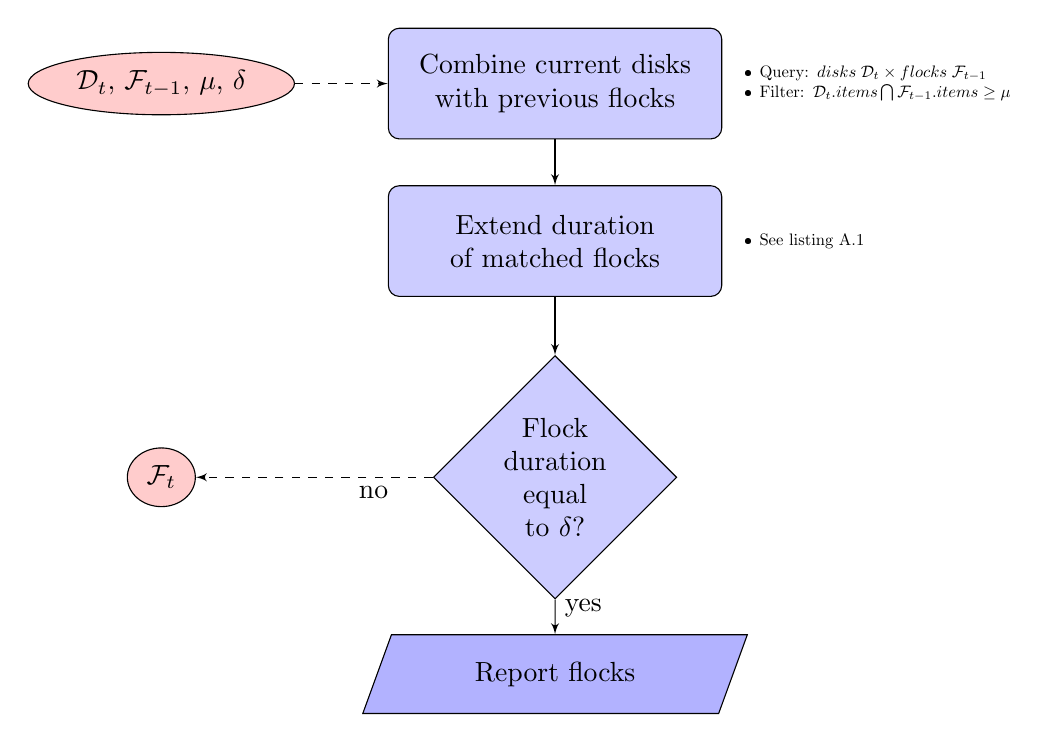
\begin{tikzpicture}[node distance = 2cm, auto]
        % Place nodes
        \node [block] (combine) {Combine current disks with previous flocks};
        \node [cloud, left of=combine] (input) {$\mathcal{D}_t$, $\mathcal{F}_{t-1}$, $\mu$, $\delta$};
        \node [block, below of=combine] (extend) {Extend duration of matched flocks};
        \node [decision, below of=extend] (decide) {Flock duration equal to $\delta$?};
        \node [io, below of=decide, node distance=2.5cm] (report) {Report flocks};
        \node [cloud, left of=decide] (output) {$\mathcal{F}_t$};
        % Info nodes
         \node [info, right of=combine] (combine_info) {
            \textbullet \hspace{0.1em} Query: $disks\;\mathcal{D}_t \times flocks\;\mathcal{F}_{t-1}$ \\
            \textbullet \hspace{0.1em} Filter: $\mathcal{D}_{t}.items \bigcap \mathcal{F}_{t-1}.items \geq \mu$ 
         };
        \node [info, right of=extend] (extend_info) { 
            \textbullet \hspace{0.1em} See listing A.1 
        };
        % Draw edges
        \path [line,dashed] (input) -- (combine);
        \path [line] (combine) -- (extend);
        \path [line] (extend) -- (decide);
        \path [line] (decide) -- node [near start] {yes} (report);
        \path [line, dashed] (decide) -- node [near start] {no}  (output);
    \end{tikzpicture}
\end{document}
